
\section{Overview}\label{sec:overview}
We introduce a model that explains most concurrency attacks we studied. 
Leveraging the model, we design a framework \xxx
to detect concurrency attacks. 
This section gives an overview of the model and architecture of \xxx.

\subsection{Preliminary}\label{sec:preliminary}

This subsection gives definitions of items we use in this paper.

\emph{\textbf{Input}}

\emph{\textbf{Bug-inducing input}} The inputs that trigger a concurrency bug. 

\emph{\textbf{Attack-inducing input}} The inputs that trigger a concurrency attack.

\emph{\textbf{Attacker thread}} The threads employed by attackers to race other thread.

\emph{\textbf{Infected thread}} The threads raced by attacker thread. In some case, a thread 
can be both infected and victim.

\emph{\textbf{Victim thread}} The threads where attacks happen. In some case, a thread 
can be both infected and victim.


\subsection{Concurrency Attack Model}\label{sec:model}

\begin{figure}
	\centering
	% \vspace{-.1in}
	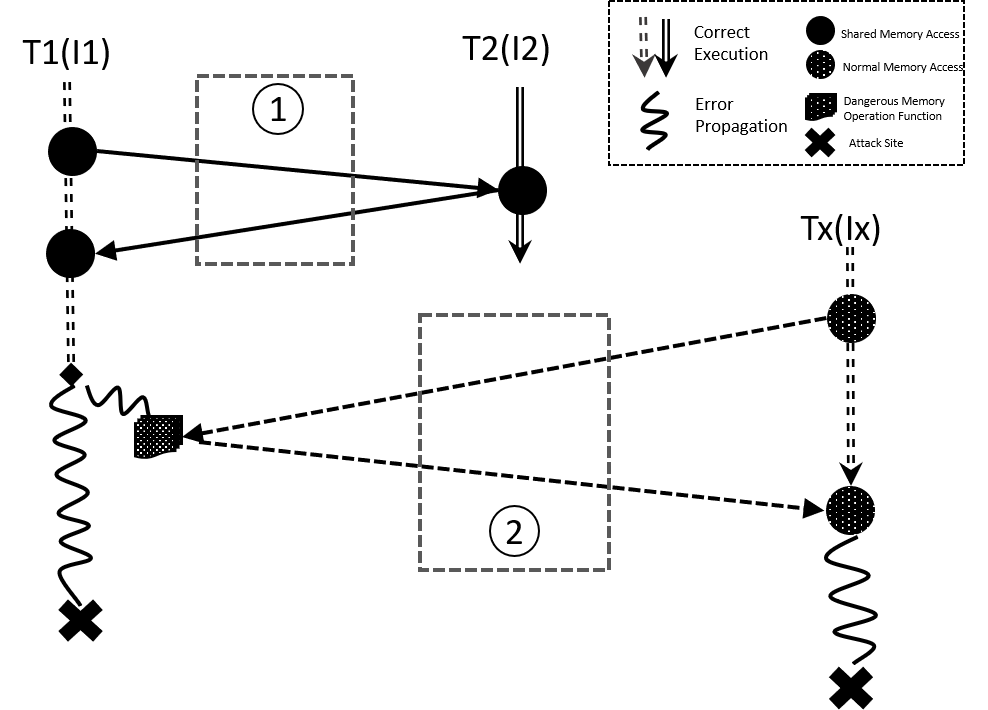
\includegraphics[width=1\columnwidth]{figures/model}
	\vspace{-.25in}
	\caption{{\em Concurrency Attack Model}} 
	\label{fig:model}
	\vspace{-0.1in}
\end{figure}




\subsection{\xxx's Architecture}\label{sec:archi}
\begin{figure*}
	\centering
	% \vspace{-.1in}
	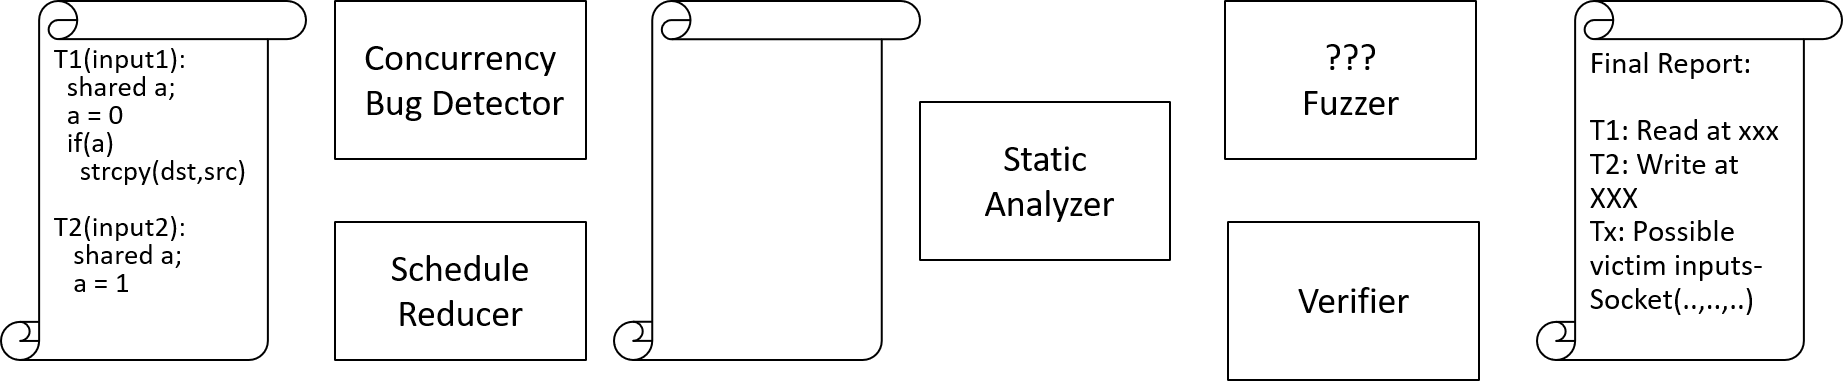
\includegraphics[width=1.8\columnwidth]{figures/archi}
	\vspace{0in}
	\caption{{\em Architecture}} 
	\label{fig:archi}
	\vspace{-0.1in}
\end{figure*}

\subsection{Detecting Example}\label{sec:example}

